\section {NFActor Overview}

\begin{figure}[!t]
  \centering
  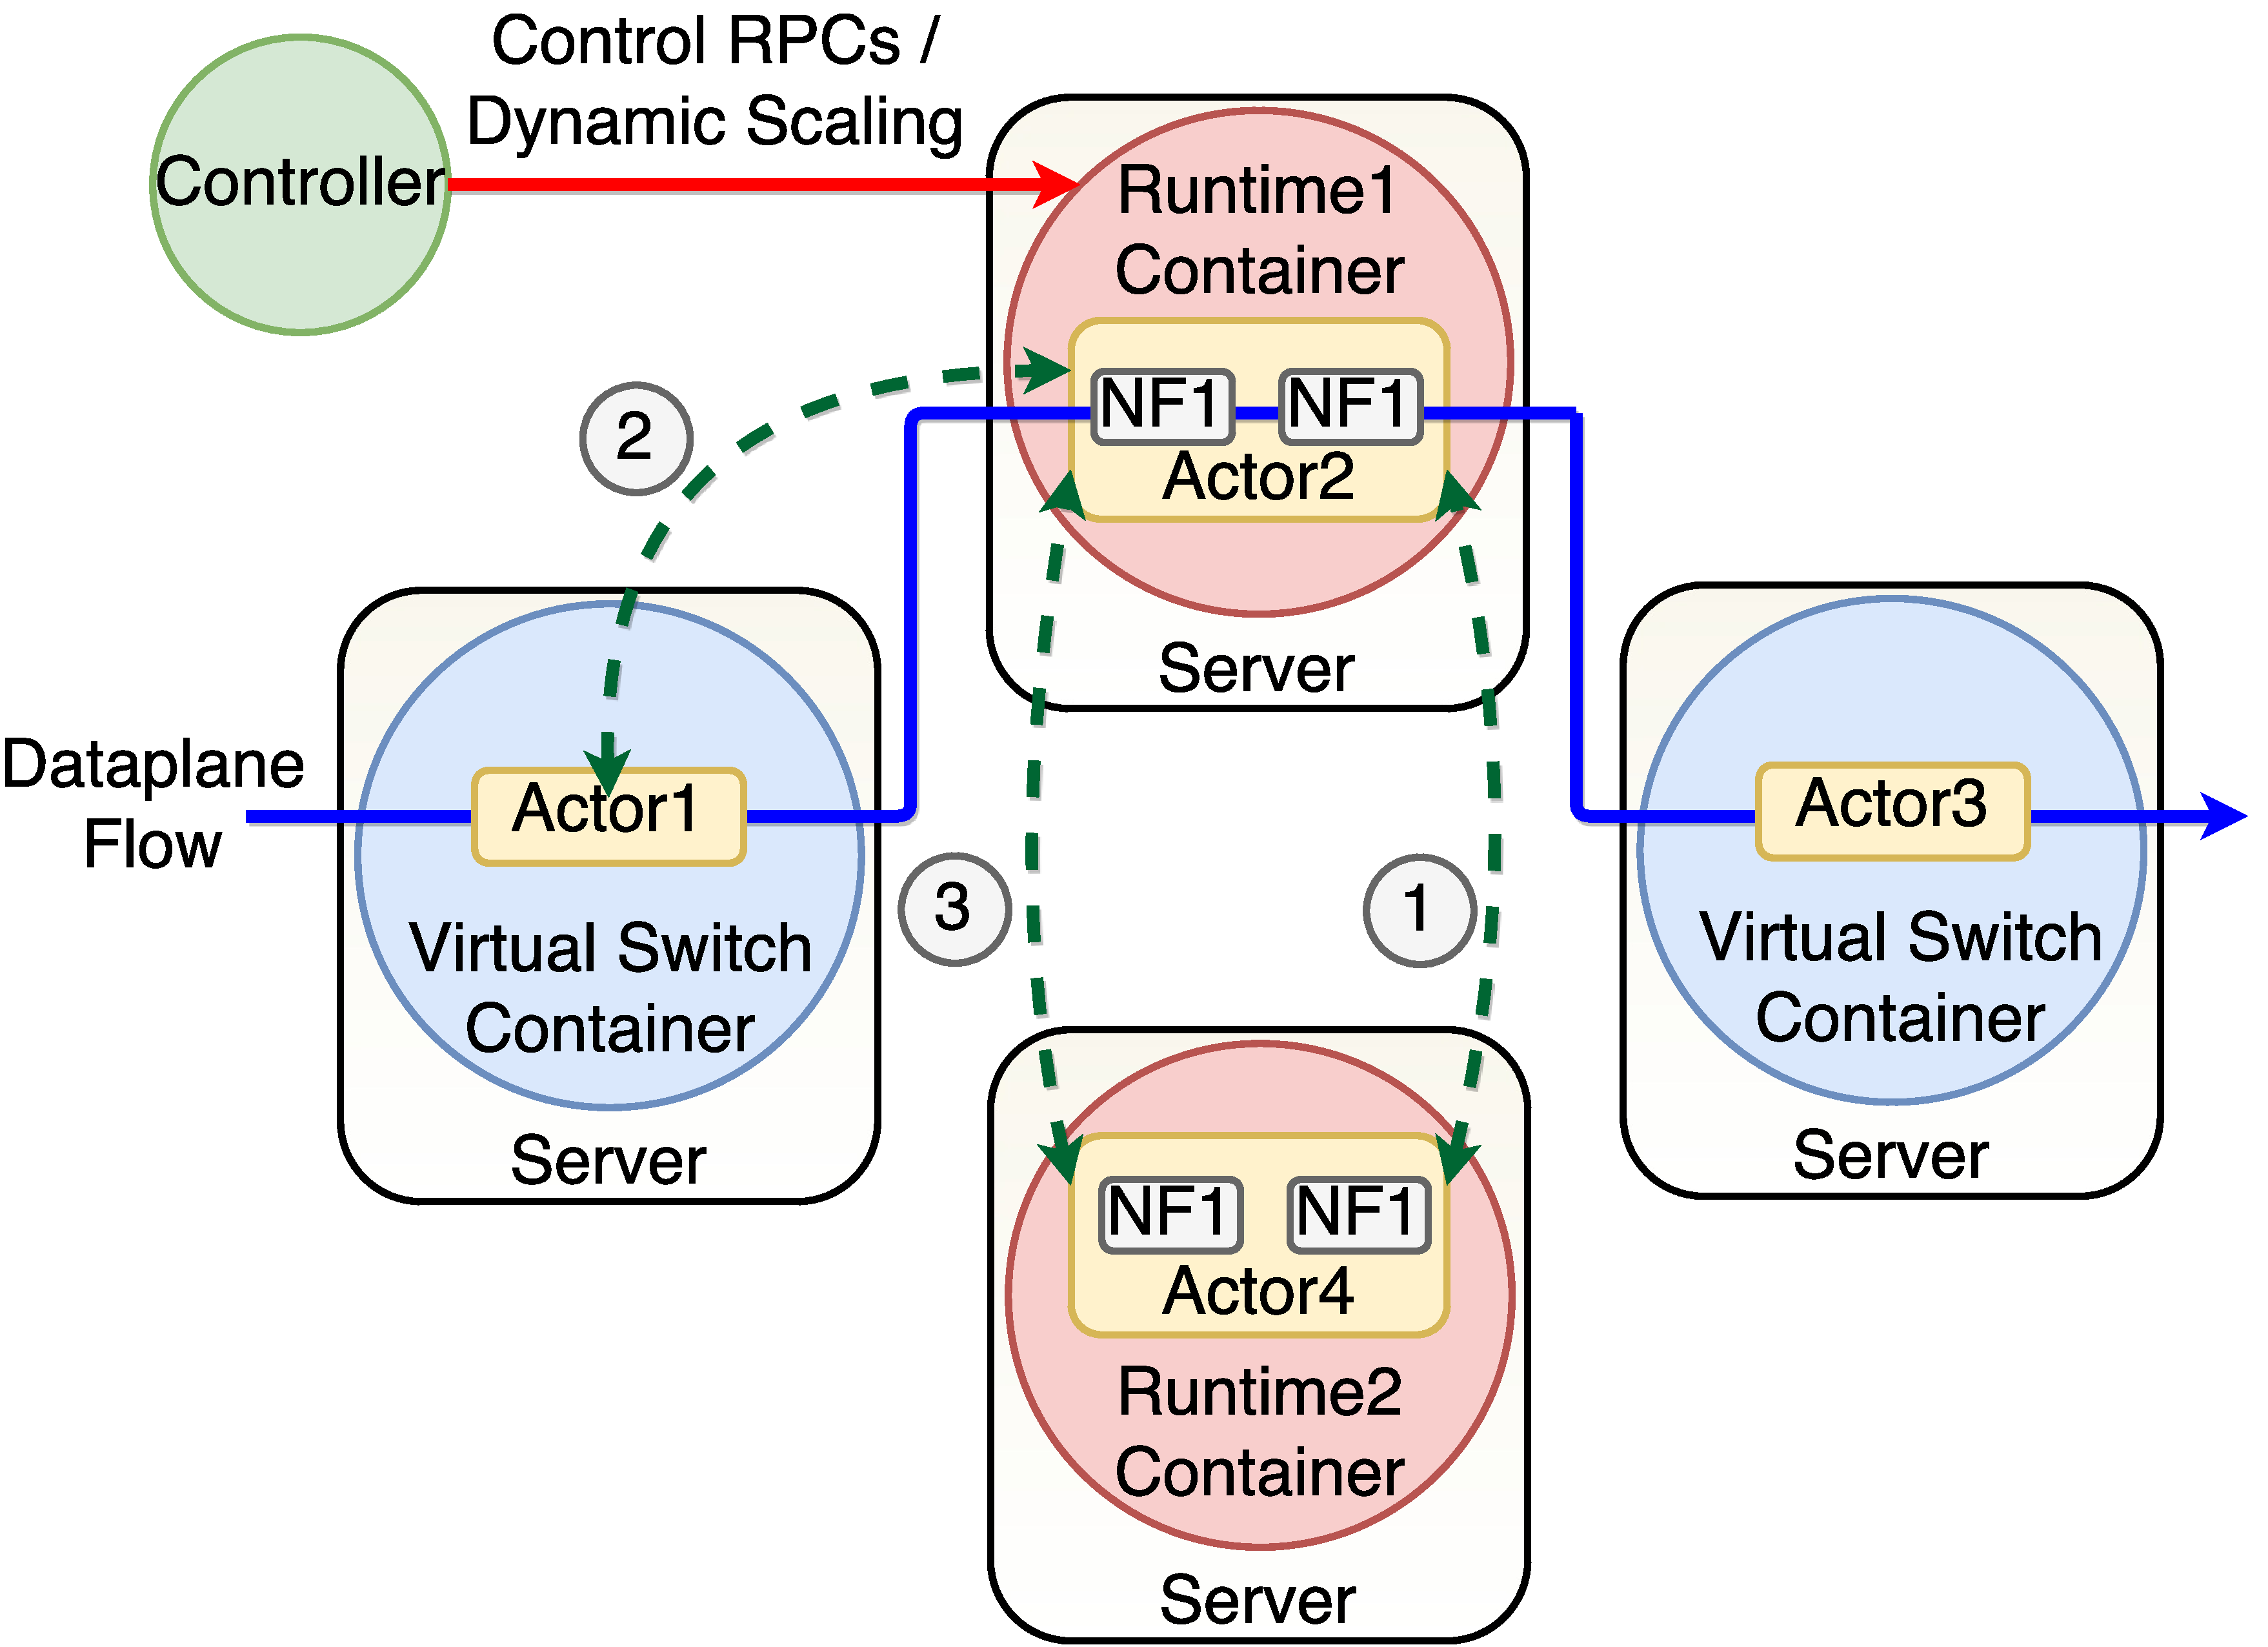
\includegraphics[width=\columnwidth]{figure/final-final-nfactor-cluster.pdf}
  \caption{An overview of NFActor framework.}
  \label{fig:runtime}
\end{figure}

Figure \ref{fig:runtime} demonstrates the basic architecture of \nfactor, consisting of a light-weight controller, input and output virtual switches and several runtime systems (referred to as \textit{runtime} in short). \ac{Both runtime and virtual switch are uniform platforms to run actors, they are executed inside containers for quick rebooting in case of failure and elastic scaling in case of overload.} \cui{Section 3 Overview: should give a clear definition on what a "runtime" is. }

%NFActor framework runs virtual switches and runtimes inside containers, so that they can be quickly rebooted in case of failure and elastically scaled in case of overload.

The incoming dataplane flows are first sent to the input virtual switch, which dispatches them to runtimes in a load-balanced fashion. \ac{Each runtime hosts a NF service chain that is determined during runtime boot phase. The runtime is designed with one-actor-one-flow principle, which decreases the overhead of passing messages among additional number of actors when processing the flow and eases the design of \nfactor's~distributed flow migration and replication.} \cui{Section 3 Overview: should briefly mention our design choice: "one-flow-one-actor".}  Therefore, when a runtime receives a new flow, it creates a new actor to process the flow. The actor loads all the required NF modules of the service chain and passes the received flow packet to these NF modules in sequence to achieve service chain processing. Once the service chain processing is finished, the actor sends the packet to an output virtual switch, where the packet is sent to its final destination.

The key feature that differentiates NFActor framework with existing works like \cite{gember2015opennf} and \cite{rajagopalan2013split} is that, resilience operations, \ie~flow migration and replication, is fully decentralized. Figure \ref{fig:runtime} demonstrates a flow migration process that migrates actor 2 on runtime 1 to runtime 2. \ac{The migration starts by actor 2 sending the first request to runtime 2. Runtime 2 launches actor 4, which is used as the migration target actor for accepting the flow packets and flow states of actor 2, before responding to actor 2. Actor 2 then sends the second request to the virtual switch, asking it to modify the output route to runtime 2. Finally, actor 2 sends its flow states in the third request to actor 4, completing the whole migration process. The details of our distributed flow migration is further illustrated in \ref{}.} \cui{The third paragraph on describing flow migration is not clear. Should make it more clear, or make it the "Section 3.1 Example" section, or cut this paragraph.}

A controller does exists in \nfactor, which is a relatively light-weighted one. It's tasks are to monitor the workload of each runtime and control dynamic scaling. It's only involvement in flow management is during the initiation phase, when it uses control RPCs to tell the flows which runtime they should migrate to.
